% !TeX spellcheck = en-US
% !TEX TS-program = pdflatex
% !TEX encoding = UTF-8 Unicode

% THIS TEMPLATE_article_for_IJET_jrnl.tex is based on
%% bare_jrnl.tex
%% V1.3
%% 2007/01/11
%% by Michael Shell
%% see http://www.michaelshell.org/
%% for current contact information.
%%
%% This is a skeleton file demonstrating the use of IEEEtran.cls
%% (requires IEEEtran.cls version 1.7 or later) with an IEEE journal paper.
%%
%% Support sites:
%% http://www.michaelshell.org/tex/ieeetran/
%% http://www.ctan.org/tex-archive/macros/latex/contrib/IEEEtran/
%% and
%% http://www.ieee.org/



% *** Authors should verify (and, if needed, correct) their LaTeX system  ***
% *** with the testflow diagnostic prior to trusting their LaTeX platform ***
% *** with production work. IEEE's font choices can trigger bugs that do  ***
% *** not appear when using other class files.                            ***
% The testflow support page is at:
% http://www.michaelshell.org/tex/testflow/


%%*************************************************************************
%% Legal Notice:
%% This code is offered as-is without any warranty either expressed or
%% implied; without even the implied warranty of MERCHANTABILITY or
%% FITNESS FOR A PARTICULAR PURPOSE!
%% User assumes all risk.
%% In no event shall IEEE or any contributor to this code be liable for
%% any damages or losses, including, but not limited to, incidental,
%% consequential, or any other damages, resulting from the use or misuse
%% of any information contained here.
%%
%% All comments are the opinions of their respective authors and are not
%% necessarily endorsed by the IEEE.
%%
%% This work is distributed under the LaTeX Project Public License (LPPL)
%% ( http://www.latex-project.org/ ) version 1.3, and may be freely used,
%% distributed and modified. A copy of the LPPL, version 1.3, is included
%% in the base LaTeX documentation of all distributions of LaTeX released
%% 2003/12/01 or later.
%% Retain all contribution notices and credits.
%% ** Modified files should be clearly indicated as such, including  **
%% ** renaming them and changing author support contact information. **
%%
%% File list of work: IEEEtran.cls, IEEEtran_HOWTO.pdf, bare_adv.tex,
%%                    bare_conf.tex, bare_jrnl.tex, bare_jrnl_compsoc.tex
%%*************************************************************************



% *** Do not adjust lengths that control margins, column widths, etc. ***
% *** Do not use packages that alter fonts (such as pslatex).         ***
% There should be no need to do such things with IEEEtran.cls V1.6 and later.
% (Unless specifically asked to do so by the journal or conference you plan
% to submit to, of course. )

%%%%%%%%%%%%%%%%%%%%%%%%%%%%%%%%%%%%%%%%%%%%%%%%%%%%%%%%%%%%%%%%%%%%%%%%%%%%%%%%%%%%%%%%%%%%%%%%%%%%%%%%%%%%%%%%%%%%%%%%%%%%
%%%%%%%%%%%%%%%%%%%%%%%%%%%%%%%%%%%%%%%%%%%%%%%%%%%%%%%%%%%%%%%%%%%%%%%%%%%%%%%%%%%%%%%%%%%%%%%%%%%%%%%%%%%%%%%%%%%%%%%%%%%%
%%%%%%%%%%%%%%%%%%%%%%%%%%%%%%%%%%%%%%%%%%%%%%%%%%%%%%%%%%%%%%%%%%%%%%%%%%%%%%%%%%%%%%%%%%%%%%%%%%%%%%%%%%%%%%%%%%%%%%%%%%%%
%%%%%%%%%%%%%%%%%%%%%%%%%%%%%%%%%%%%%%%%%%%%%%%%%%%%%%%%%%%%%%%%%%%%%%%%%%%%%%%%%%%%%%%%%%%%%%%%%%%%%%%%%%%%%%%%%%%%%%%%%%%%

\documentclass[journal,a4paper,twoside]{IEEEtran}

\def\IEEEkeywordsname{Keywords}
\usepackage{ragged2e}



\usepackage[english]{babel}
\usepackage{csquotes}
\usepackage[citestyle=numeric-comp,bibstyle=ieee,%
backend=biber,sortcites]{biblatex}
\renewbibmacro*{bbx:savehash}{} % Remove annoying dash
\addbibresource{bib/bib-art1.bib}
\addbibresource{bib/manual-biblatex.bib}



\usepackage{url}

\usepackage{graphicx}
\usepackage{epstopdf}

\hyphenation{op-tical net-works semi-conduc-tor}
\usepackage{balance}

\usepackage[bottom]{footmisc}
\usepackage{fancyhdr}
\usepackage{multicol}
\usepackage[
type={CC},
modifier={by},
version={4.0},
]{doclicense}

\usepackage{todonotes}

\widowpenalty=300000
\clubpenalty=300000

%%%%%%%%%%%%%%%%%%%%%%%%%%%%%%%%%%%%%%%%%%%%%%%%%%%%%%%%%%%%%%%%%%%%%%%%%%%%%%%%%%%%%%%%%%%%%%%%%%%%%%%%%%%%%%%%%%%%%%%%%%%%%
%%%%%%%%%%%%%%%%%%%%%%%%%%%%%%%%%%%%%%%%%%%%%%%%%%%%%%%%%%%%%%%%%%%%%%%%%%%%%%%%%%%%%%%%%%%%%%%%%%%%%%%%%%%%%%%%%%%%%%%%%%%%%
% EDITOR SECTION (Please Do not change)

%IJET first page header
%%% FIXME TODO
\newcommand{\YEAR}{2020}
\newcommand{\VOLUME}{66}
\newcommand{\NUMBER}{1}
\newcommand{\PAGES}{1--6}
\newcommand{\RECEIVEDATE}{October 10, 2019}
\newcommand{\REVISIONDATE}{January, 2020}
\newcommand{\DOI}{DOI: 10.24425/ijet.2019.126xxx}

\usepackage{fancyhdr}
\lhead
{
	\begin{picture}(0,0)
	\put(0,-35){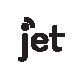
\includegraphics{fig/logo_first_page}}
	\put(30,-22){\scriptsize\MakeUppercase{INTL Journal of Electronics and Telecommunications, \YEAR, Vol. \VOLUME, no. \NUMBER, pp. \PAGES}}
	\put(30,-30){\scriptsize{Manuscript received \RECEIVEDATE; revised \REVISIONDATE.$\qquad\,\quad\qquad$\DOI}}
	\end{picture}
}
\chead{}
\rhead{}
\lfoot
{
	\begin{picture}(0,0)
	\put(0,0){\doclicenseImage[imagewidth=5.5em]}
	\put(65,12){\scriptsize $\copyright$
	{\scriptsize The Author(s). This is an open-access article distributed under the terms of the Creative Commons Attribution License (CC BY 4.0,}}
	\put(65,2){\scriptsize {\href{https://creativecommons.org/licenses/by/4.0/}{https://creativecommons.org/licenses/by/4.0/}), which permits use, distribution, and reproduction in any medium, provided that the Article is properly cited.}}
	\end{picture}}

\cfoot{}
\rfoot{}
\renewcommand{\headrulewidth}{0pt}
\renewcommand{\footrulewidth}{0pt}

%\begin{multicols}{1}
%\fancyfoot[L]{\doclicenseImage[imagewidth=4em] $\copyright$
%	{\scriptsize The Author(s). This is an open-access article distributed under the terms of the Creative Commons Attribution License (CC BY 4.0, \href{https://creativecommons.org/licenses/by/4.0/}{https://creativecommons.org/licenses/by/4.0/}), which permits use, distribution, and reproduction in any medium, provided that the Article is properly cited.}}
%\pagestyle{fancy}
%\end{multicols}

\setcounter{page}{1}

\linespread{1.02}

%%%%%%%%%%%%%%%%%%%%%%%%%%%%%%%%%%%%%%%%%%%%%%%%%%%%%%%%%%%%%%%%%%%%%%%%%%%%%%%%%%%%%%%%%%%%%%%%%%%%%%%%%%%%%%%%%%%%%%%%%%%%%
%%%%%%%%%%%%%%%%%%%%%%%%%%%%%%%%%%%%%%%%%%%%%%%%%%%%%%%%%%%%%%%%%%%%%%%%%%%%%%%%%%%%%%%%%%%%%%%%%%%%%%%%%%%%%%%%%%%%%%%%%%%%%
% AUTHOR SECTION ( This is a skeleton file demonstrating the use of TEMPLATE_article_for_IJET_jrnl.tex)
%%pdfinfo is document information - this information makes pdf much more usefull for search engines;
%%clik ctr+D on open pdf document and check information about this document

%TODO
\pdfinfo {
	/Author (Mikołaj Kowalski, Wojciech Mazurczyk)
	/Title (Towards mutual routing security -- a review)
	/Keywords (Routing protocols, Network security, Telecommunication network reliability, Wide area networks)
}


%%%%%%%%%%%%%%%%%%%%%%%%%%%%%%%%%%%%%%%%%%%%%%%%%%%%%%%
% BODY OF THE ARTICLE

\begin{document}
%
% paper title
% can use linebreaks \\ within to get better formatting as desired

\title{\vspace{1cm} Towards mutual routing security -- a review}
%\title{\vspace{1cm} Mutual routing security with RPKI\\ -- protect your peers just like in pandemic time}
%
%
% author names and IEEE memberships
% note positions of commas and nonbreaking spaces ( ~ ) LaTeX will not break
% a structure at a ~ so this keeps an author's name from being broken across
% two lines.
% use \thanks{} to gain access to the first footnote area
% a separate \thanks must be used for each paragraph as LaTeX2e's \thanks
% was not built to handle multiple paragraphs
%

\author{Mikołaj~Kowalski, Wojciech~Mazurczyk% <-this % stops a space
	\thanks{This work was supported by the grant No. xxxxxx ”Doktorat wdrożeniowy” by Ministerstwo Edukacji i Nauki.}% stops a space
	\thanks{M.~Kowalski is with Faculty of Electronics and Information Technology, Warsaw University of Technology, Poland (e-mail: 6796@pw.edu.pl).}% <-this % stops a space
	\thanks{Professor W.~Mazurczyk is with Faculty of Electronics and Information Technology, Warsaw University of Technology, Poland (e-mail:  wmazurcz@(NOSPAM)elka.pw.edu.pl).}% <-this % stops a space
}


% note the % following the last \IEEEmembership and also \thanks -
% these prevent an unwanted space from occurring between the last author name
% and the end of the author line. i.e., if you had this:
%
% \author{....lastname \thanks{...} \thanks{...} }
%                     ^------------^------------^----Do not want these spaces!
%
% a space would be appended to the last name and could cause every name on that
% line to be shifted left slightly. This is one of those \L{}aTeX things". For
% instance, "\textbf{A} \textbf{B}" will typeset as \k{A} B" not \k{A}B". To get
% \k{A}B" then you have to do: "\textbf{A}\textbf{B}"
% \thanks is no different in this regard, so shield the last } of each \thanks
% that ends a line with a % and do not let a space in before the next \thanks.
% Spaces after \IEEEmembership other than the last one are OK (and needed) as
% you are supposed to have spaces between the names. For what it is worth,
% this is a minor point as most people would not even notice if the said evil
% space somehow managed to creep in.



% The paper headers
%\markboth{Journal of \LaTeX\ Class Files,~Vol.~6, No.~1, January~2007}%
%{Shell \MakeLowercase{\textit{et al.}}: Bare Demo of IEEEtran.cls for Journals}%
%
\markboth{}{}
%
% The only time the second header will appear is for the odd numbered pages
% after the title page when using the twoside option.
%
% *** Note that you probably will NOT want to include the author's ***
% *** name in the headers of peer review papers.                   ***
% You can use \ifCLASSOPTIONpeerreview for conditional compilation here if
% you desire.




% If you want to put a publisher's ID mark on the page you can do it like
% this:
%\IEEEpubid{0000--0000/00\$00.00~\copyright~2007 IEEE}
% Remember, if you use this you must call \IEEEpubidadjcol in the second
% column for its text to clear the IEEEpubid mark.



% use for special paper notices
%\IEEEspecialpapernotice{(Invited Paper)}

%IJET header for even and odd pages (Caution: with exeption the first page)
\maketitle
\thispagestyle{fancy}%
\markboth{M.~Kowalski, W.~Mazurczyk}{Example of Article for International Journals of Electronics and Telecommunications} %TODO
%


% ABSTRACT

\begin{abstract}
Historically, the inter-domain routing security had to be established based on trust, due to poorly designed BGP protocol. This approach is insufficient, as seen in practice numerous times. To prevent this, new kind of security measures were proposed and thus are needed to be implemented on Internet's majority Autonomous Systems.

This article covers the current threat landscape and existing taxonomy of attack vectors on routing layer, with the analysis of incident types and giving the detailed breakdown in incidents classification. In order to ..., best/new unified taxonomy will be proposed./  \todo[inline]{czy review to miejsce na nowe taksonomie?  czy analiza porownawcza jest wystarczajaca?}

The review contain comprehensive protective measures study, with current techniques efficiency as well as caveats. Authors also dissect most promising development plans for new and existing countermeasures.

However, due to current Resource Public Key infrastructure system design, safeguard mechanisms of routing security are based on mutual protection. This causes the chicken or the egg problem. Authors will try to explain slow adoption rate and some estimates will be given. 
\end{abstract}


% KEYWORDS

\begin{IEEEkeywords}
Routing protocols, Network security, Telecommunication network reliability, Wide area networks
\end{IEEEkeywords}

\IEEEpeerreviewmaketitle

% FIRST section - INTRODUCTION

\section{Introduction to routing security}


\IEEEPARstart{A}{utonomous Systems} (ASes) are main, essential entity in today's Internet. As defined in \cite{rfc1930}, "an AS is a connected group of one or more IP prefixes run by one or more network operators which has a SINGLE and CLEARLY DEFINED routing policy". When routing policy is configured and accepted by adjacent ASes (peers) traffic is allowed to flow. If a traffic is traversing in an unintended fashion (conflicting with the routing policy), one can call a \emph{routing incident}.

Routing incidents has been a subject of a study for over a two decades now. In a plethora of research papers, we have seen \cite{Chakrabarti2002} there are too generic or \cite{Schlamp2016} too formal. However, there are some work that in our opinion maintain the perfect balance. We in detail discuss \cite{rfc7908} taxonomy that has been defined to serve as a common definition for Internet users and operators community and \cite{Sermpezis2018a} which is based on novel approach. To complement this great works, we propose some additional common metrics, to provide a unified characterization of routing incidents.

Detailed breakdown of incident types and enumeration of different scenarios is presented in section \ref{def:tax}.
\todo[inline]{todo po napisaniu tego par}

Threat landscape and risk analysis are available in \ref{def:impact}.
\todo[inline]{todo po napisaniu tego par}

There are well defined means of protection which mitigates impact for these attacks. Main division factor that should differentiate them is \emph{passive} -- traditionally used as basic BGP \emph{hygiene} intended for verifying the trust of a peer or traffic engineering tricks, and \emph{proactive} means -- new generation technologies that guarantee an incident will not happen. Both categories are described in sections \ref{protect:filtering} and \ref{protect:rov},\ref{protect:path}, respectively.

In section \ref{now:slow} author summarizes the RPKI implementation global progression and tries to give a prognosis on future efforts. To give complete view, section \ref{now:caveats} describes some unwanted scenarios and threat that RPKI introduces. The section \ref{now:future} provides the overview on future development directions.

Section \ref{conclusion} states authors' conclusions.



%%%%%%%%%%%%%%%%%%%%

% !TEX root = ../main.tex

\section{Routing incidents taxonomy -- problem definition}
\label{def}
In general, the routing incident is undesirable routing system change, to the state that it is no longer operational or working at suboptimal capacity.



There are several different metrics that can be used to classify routing incident, in this work we will explore criteria/benchmarks such as:
\begin{description}
    \item[\textbf{type}] most important, incident ought to be pinned to a category that ensure unambiguous classification. More on that in \ref{def:tax}
	\item[\textbf{intent}] an incident may originate from intentional, malicious action (so called attack). If done on purpose, possible causes are interception of traffic to espionage, credential theft, censorship or denial of service (downtime, outage) specific website or company. In contrary, erroneous configuration that is result of human mistake, sometimes called \emph{fat finger} mistake, does not have an ultimate agenda.
	\item[\textbf{scale}] the targeted incident might be for one prefix only, but sometimes there will be plenty prefixes involved
	\item[\textbf{impact}] there are multiple factors in this metric, so this will be discussed in \ref{def:impact}
	\item[\textbf{duration}] usually, errors impacting substantial amount of networks or users are corrected in a timely manner, but some small incidents may last weeks unnoticed
	\item[\textbf{range}] some incident will be accepted only by peer AS, but some of them will propagate globally (to the DFZ)
\end{description}

\subsection{Routing incidents characteristics and taxonomy}
\label{def:tax}
The most basic division of routing incidents are \emph{BGP Hijacks} and \emph{Route Leaks}. In this paper we present ... (state of the art/ best in our opinion?) taxonomy. 

\subsubsection{Route leaks}
\label{def:tax:rl}
As defined in \cite{rfc7908}, route leak is propagation of (single or multiple) routing announcement beyond their intended scope, which is defined by routing policy, implemented by a set of redistribution filters. Route leaks are typically not malicious, most often an effect of configuration mistake. 

Most common scenario for leak is when a multihomed stub AS re-advertise a prefix from one of it's transit providers to another. The second provider won't detect a leak and propagate the route further. However, IETF suggest more detailed classification of leaks:

\begin{figure}[ht]
    \begin{center}
   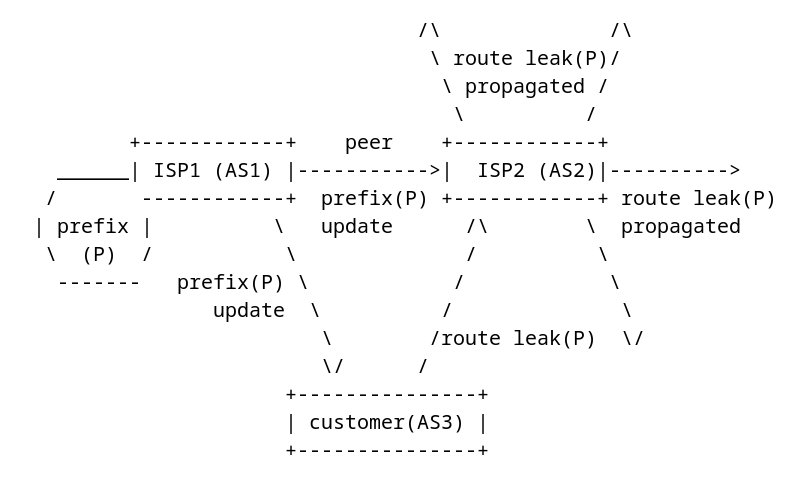
\includegraphics[width = 0.8\linewidth]{./img/route-leak-topology.png}
    \end{center}
    \caption{Route Leak topology \cite{rfc7908} (do przerysowania?) \label{fig:routeleak}}
\end{figure}

\begin{itemize}
    \item \textbf{Type 1: Hairpin Turn with Full Prefix} -- most common case, that makes the stub network that leaked a prefix a transit network. Leak is usually successful, as transit networks usually accept prefixes from their customers. The traffic will reach the destination if stub network will be able to process higher volume of traffic. 
    \item \textbf{Type 2: Lateral ISP-ISP-ISP Leak} -- when ISP's are peering, they should announce only prefixes of their customers. Type 2 takes place when an ISP is propagating prefix of the another ISP whom peering agreement was established.
    \item \textbf{Type 3: Leak of Transit-Provider Prefixes to Peer} -- this type is about propagating prefixes from transit provider to lateral network, effectively providing transit service to the peer.
    \item \textbf{Type 4: Leak of Peer Prefixes to Transit Provider} -- comparing to Type 3, this has the flow in opposite direction . However, it is more dangerous, as it may hurt the peer when the \textsc{AS-Path} is shortened 
    \item \textbf{Type 5: Prefix Re-origination with Data Path to Legitimate Origin} -- offending multihomed AS announces learnt prefix but without original \textsc{AS-Path}. This case is similar to \textbf{Type-0, Exact Prefix, MitM Prefix Hijack} classified in \cite{Sermpezis2018a}, but it assumes that the prefix ought to be learnt from upstream ISP. 
    \item \textbf{Type 6: Accidental Leak of Internal Prefixes and More-Specific Prefixes} -- this type is different, as the prefixes in leak are originating from within offending AS. This is a common issue, typically a badly configured export policy, insufficient aggregation or weak outbound filters. More specific prefixes should not be present in DFZ when a less-specific route exists. In contrast to \textbf{Type-0 Sub-prefix BGP Hijack}, offending AS owns prefixes that are announced.  
\end{itemize}

\subsubsection{BGP Hijacks}
\label{def:tax:hj}
Hijack event is when the adversary Autonomous System illegitimately advertise an IP prefix (or part of it) belonging to other AS. The advertisement needs to propagate towards other BGP speakers if hijack is considered to be successful.

Authors in \cite{Sermpezis2018a} proposed a very detailed taxonomy, with three split categories.  The \emph{affected prefix} can be the same as rightfully originated (\textbf{Exact Prefix Hijack}) or more-specific (\textbf{Sub-Prefix Hijack}), but also not currently advertised (\textbf{Squatting Hijack}) by the victim. Furthermore \emph{AS-Path announced} might be simply substituted for hijacker ASN only (\textbf{Type-0 Hijack}) or modified with victim ASN first and hijacker ASN last in the path (\textbf{Type-N Hijack}). Moreover when the \textsc{AS-Path} is not modified, one should distinguish \textbf{Type-U Hijack}. The third category concerns data-plane traffic handling when a hijack takes place. Possible actions that can be taken by adversary are: \textbf{blackhole} when the traffic is simply dropped, \textbf{man-in-the-middle} for connection eavesdropping or manipulating, or \textbf{imposture} when adversary mimics the victim services and an interaction with legitimate hosts takes place.


%\subsection{Routing incidents characteristics} 

\subsection{Impact of routing incidents}
\label{def:impact}
\subsubsection{BGP Hijacks}
\label{def:impact:hj}
When a Autonomous System attempt Hijack it may affect availability, integrity, and confidentiality of communications in the victim network. The impact depends mostly on the intent of the incident, closely related to the adversary agenda. However, to break down to technical indicators, lets analyse it by the incident type data-plane traffic handling. 

For blackhole there is availability problem for victim's network and possible full outage (denial of service situation). It is similar in effect to data-plane DoS attack, but it's less expected and harder to defend to. 

When considering man-in-the-middle the adversary is creating malicious BGP Hijack it focused on getting the data and keeping the connection intact. Use cases include credential theft, data manipulation .... <TODO>

The most advanced technique is impersonating victim's servers. <TODO>


\subsubsection{Route leaks}
\label{def:impact:rl}
With Route Leaks, <TODO>

Route leak will cause a redirection of traffic to the different path that it was intended. This may or may not result in overloading some network equipment and network links or blackholing the traffic altogether. 

\subsection{Measuring attack impact in the wild}
\label{def:measurement}
Hijacks sometimes have a severe and lasting impact. While it is relatively easy to monitor the state of routing in the Internet's control-plane thanks to initiatives like RIPE RIS\footnote{\url{https://ris-live.ripe.net/}} and software build on top of it or Qrator Radar\footnote{\url{https://radar.qrator.net/}} directly detecting some kind of routing incidents, it is difficult to verify real impact -- users affected and financial losses as companies tend to not disclose such details. 

However, there has been attempt to check real impact of routing incidents. As surveyed among 75 networks from NANOG and RIPE mailing list subscribers in \cite{Sermpezis2018}, 41\% of the operators reported that their organization has been a victim of a hijack in the past. \textquote{The vast majority (76\%) expects the impact of a hijack to last for a long time (few hours or more), while opinions are divided on whether the hijack will affect a few or many of their services/clients, indicating that there are concerns both for extended (e.g.route leaks) and limited/targeted (e.g. malicious attacks) hijacks. (...) More than 57\% of hijacks lasted more than an hour, while 25\% lasted more than a day; around 28\% are short-term hijacks, lasting a few minutes (14.3\%) or seconds (14.3\%). }





\subsection{Incident examples}

MyEtherWallet, provider for Etherum cryptocurrency wallets has been attacked by a BGP hijack on April 24th, 2018\cite{Brandom2018}. The attack was not carried directly at MyEtherWallet, but instead on Amazon Web Services' DNS infrastructure. Worth noting is that AWS DNS was not compromised, but the AWS Route 53 prefix space was the subject of hijack. The resulting outcome was \$365,000 stolen in ETH, in spite of users being warned of self-signed TLS certificate. The attacker was announcing more-specific prefixes (\textbf{sub-prefix hijack}) and running \textbf{man in the middle} proxy for DNS traffic. The cryptocurrency website was \textbf{impersonated}.

Telekom Malaysia (AS4788) and Level3 (AS3549) incident was massive \textbf{Type 4} and \textbf{Type 6} route leak. As described in \cite{Toonk2015}, more than 176 000 prefixes learnt from peering session in DEC-IX and more-specific client prefixes were leaked to upstream provider. This resulted in huge amount of traffic being directed to AS4788 which caused network overload also for Level3. Typical symptoms like packet loss and RTT increase was observed. 

Another case of among many route leak incidents resulted in outage of AWS and Amazon services unavailability. As described by researcher from ThousandEyes in \cite{Kephart2015}, AS33083 announced AWS' prefixes to it's transit provider AS5580. This announcement wasn't in the path before, so the prefix leak is of \textbf{Type 4} \ref{def:tax:rl}. The leak has affected cloud services and therefore multiple companies.





\subsection{Other techniques accompanying routing attacks}
\label{def:mitm}
\subsubsection{Acquisition of Bogus TLS certificate using BGP sub-prefix interception}
Most of the times, to perform a successful attack an adversary is required to do some kind of MiTM attack.
For example, the simplest way to redirect the traffic is to redirect DNS queries and spoof the DNS response.
An attacker will be available to issue a valid TLS certificate, as he will be able to pass all checks that CA is using to verify remote side.
\cite{Gavrichenkov2015}


As presented in \cite{Gavrichenkov2015}, further executed and measured in \cite{BirgeLee2017},\cite{BirgeLee2018}, there is a possibility to issue a valid certificate that should not be issued. The mechanism presented shows a bug in CA's verification procedure, however using BGP routing attack can exploit this bug, leading to further target impersonating by the attacker.
Researchers suggest two countermeasures for CA's: \emph{Multiple Vantage Point Verification} and \emph{Monitoring BGP Route Age}.

\subsubsection{Excessive BGP ASPath prepending increase risk of successful routing incident}
Many network operators use prependig as a traffic shaping tool, because by the design of the BGP protocol, router should choose the shorter, not prepended route (assuming that other criteria are equal). Prepending is a common practice in the Internet and if done correctly if may be used beneficially for traffic steering. However, researchers point out\cite{Madory2019} that wrong usage called \textbf{prepend-to-all} has been observed in over a 8\% prefixes of IPv4 Global Routing Table. This practice is all about advertising the prefix with multiple origin ASN repetition in the AS Path. This opens a vulnerability that if another AS will announce (mistakenly or on purpose) same prefix with shorter AS Path, traffic will be redirected from it's usual path with consequences as described in \ref{def:impact:rl}. 


%%%%%%%%%%%%%%%%%%%%5

% !TEX root = ../main.tex

\section{Safeguards}
\label{protect}
TODO

preventive (mitigate risk) -- vs post-incidental


\subsection{Traditional protection}
\label{protect:filtering}
bgp filtering,classical approach

 Considerations in Validating the Path in BGP \cite{rfc5123}
\subsection{Route Origin Validation}
\label{protect:rov}

\subsection{Full Path Validation}
\label{protect:path}
aka {BGP} AS\_PATH attribute


BGPSec \cite{rfc8205} \cite{rfc8206}

Please see \ref{now:future:path} for more on Path Validation


%%%%%%%%%%%%%%%%%%%%%%

% !TEX root = ../main.tex

\section{Current state of affairs and future work}
\label{now}

In previously cited survey study \cite{Sermpezis2018}, most of the network operators (71\%) answered that they have not deployed RPKI as a proactive defense mechanism in their networks \ref{fig:usagerpki}; very few (12\%) use the full functionality of RPKI (Route Origin Authorization -- ROA and Route Origin Validation -- ROV). ROA is used by 15\% of networks.

\begin{figure}[ht]
 \begin{center}
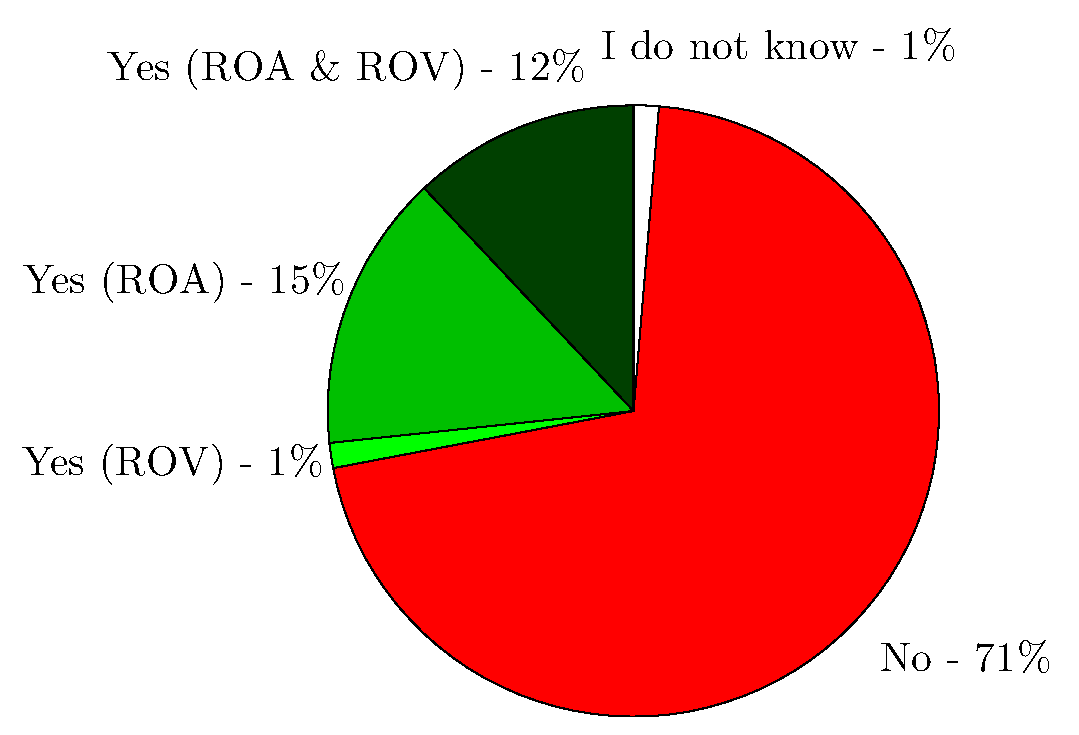
\includegraphics[width = 0.8\linewidth]{./fig/fig_survey_use_RPKI}
 \end{center}
 \caption{Usage of RPKI based on survey by \cite{Sermpezis2018}} \label{fig:usagerpki}
\end{figure}

However, these number seems to be changing, as cam be seen on \ref{fig:rpki-rov} and \ref{fig:rpki-roa}.

\begin{figure}[ht]
	\begin{center}
   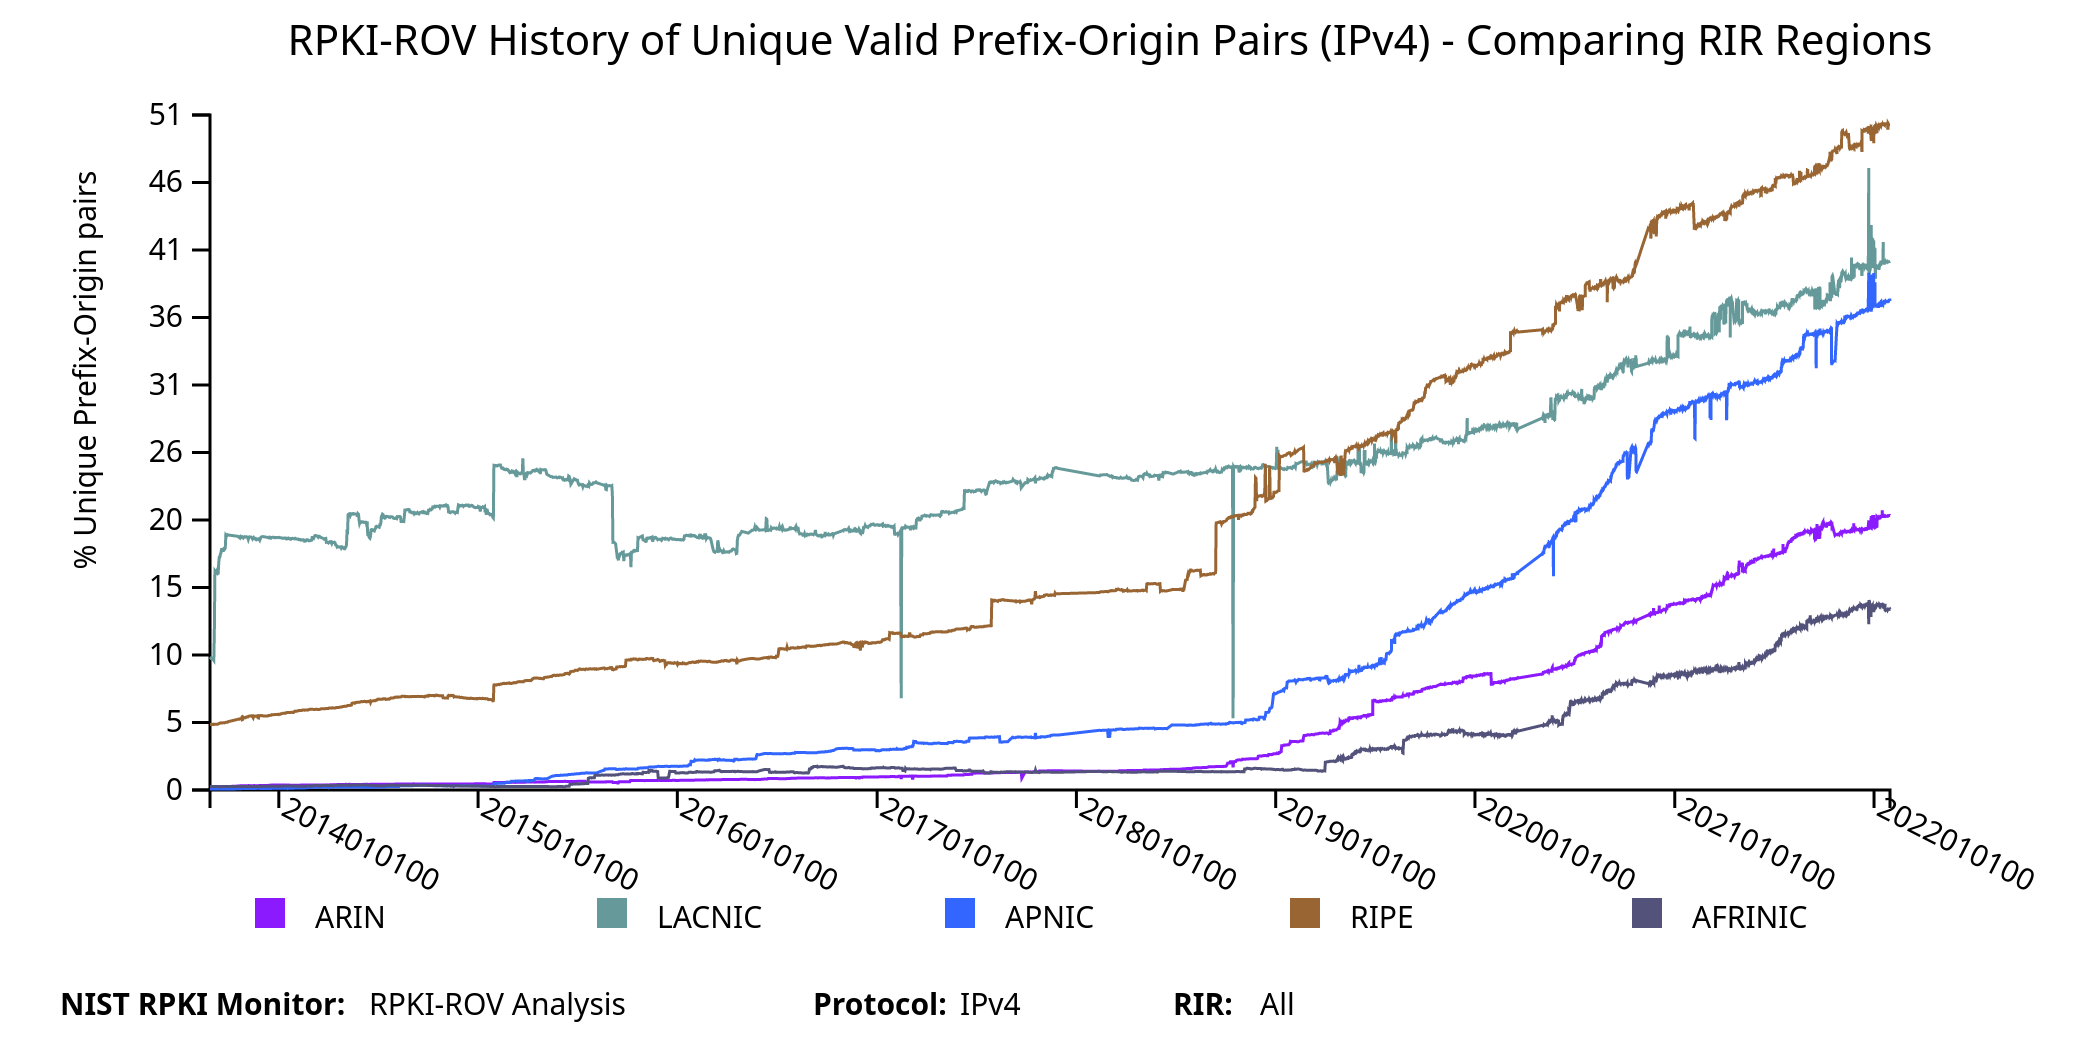
\includegraphics[width = 1\linewidth]{./img/RPKIROV_20220130.png}
	\end{center}
	\caption{A percent of the total count unique announced Prefix-Origin pairs with prefixes in the corresponding RIR. Source: NIST RPKI Monitor \label{fig:rpki-rov}}
\end{figure}
\begin{figure}[ht]
	\begin{center}
   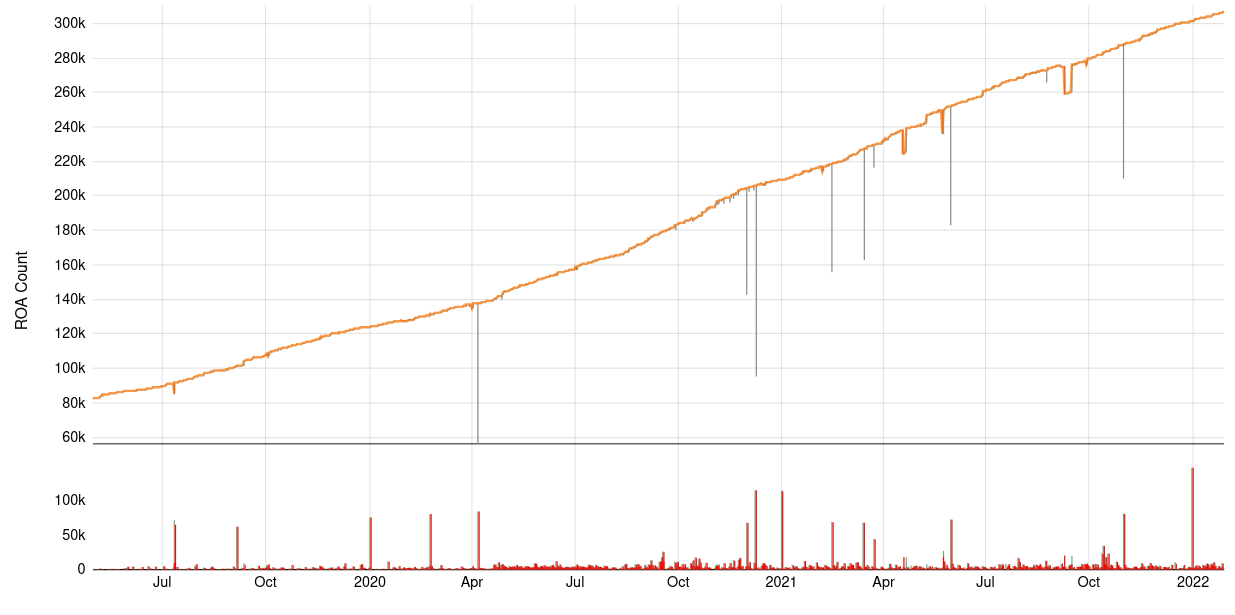
\includegraphics[width = 1\linewidth]{./img/ROA-history.png}
	\end{center}
	\caption{Total count of ROA over time. Source: Cloudflare RPKI Portal\label{fig:rpki-roa}}
\end{figure}
\subsection{Slow adoption}
\label{now:slow}



\subsubsection{Lack of awareness}
TODO

MANRS is doing a great job\cite{Robachevsky2020}

\subsubsection{Technical difficulties}
Researches in \cite{Sermpezis2018} points that
\textquote{deployment lags mainly due to RPKI's limited adoption and little security benefits, but also due to the increased CAPEX and OPEX costs, and increased complexity and processing overhead associated with the protocol mechanisms. Therefore, about 60\% of the operators  resort to other mechanisms and practical defenses to protect their networks against BGP hijacks.} For detailed breakdown of adoption slowiness causes, see fig. \ref{fig:notrpkireasons}.


 \begin{figure}[h]
 	\begin{center}
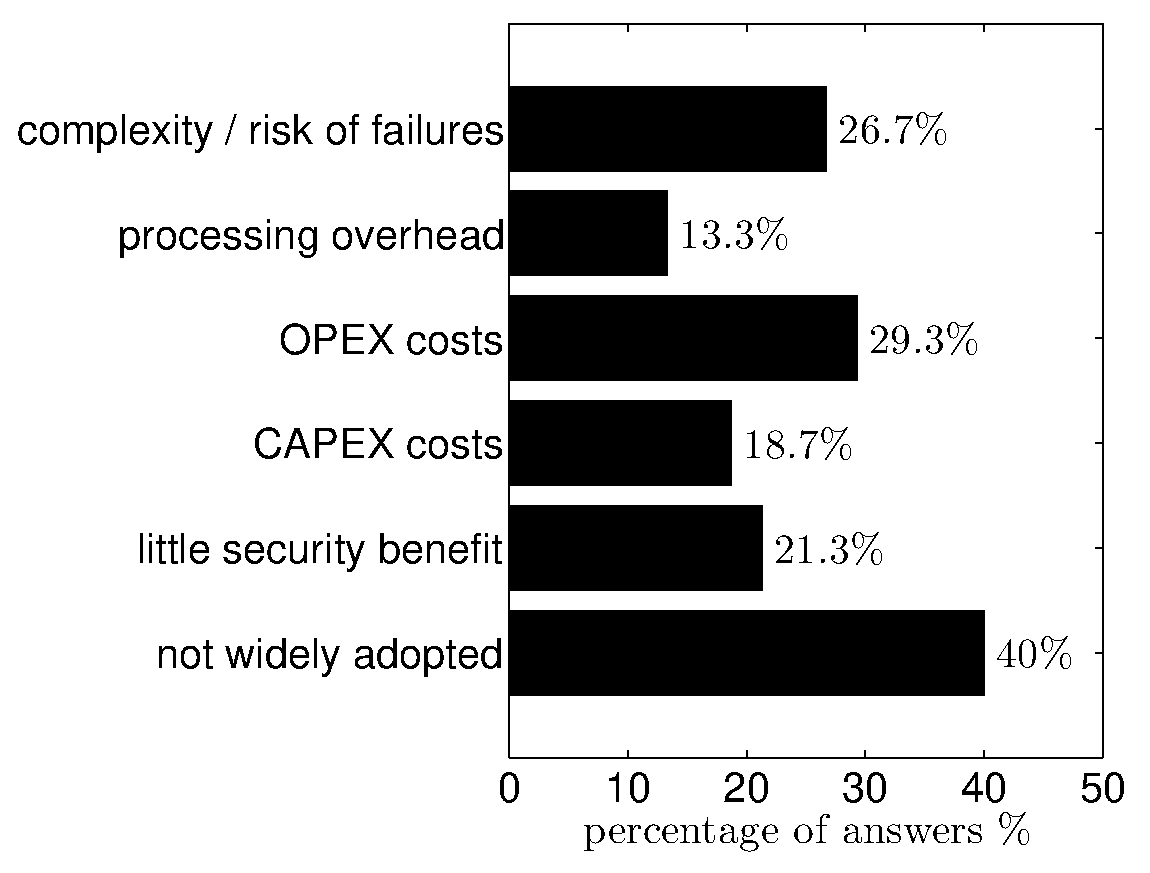
\includegraphics[width = 1\linewidth]{./fig/fig_survey_reasons_rpki}
 	\end{center}
 	\caption{Main reasons not using RPKI based on survey by \cite{Sermpezis2018}} \label{fig:notrpkireasons}
 \end{figure}

\subsubsection{Legal issues}
Widespread RPKI adoption may be limited due to specific status on ARIN's terms and conditions for RPKI repository.
Third parties who wish to validate BGP routes had to agree \emph{Relying Party Agreement}.
As a result, most RP validating software does not come with ARIN TAL embedded by default.


This has a direct effect on ARIN members in North America -- Route Origin Validation on ARIN AS' has been significantly lower. Almost 80\% of those AS engaging in ROV omit the ARIN TAL, has been proofed by \cite{CartwrightCox2018}.

In the beginning of 2019, the gap between ARIN's ROA only grew. This state of affairs was criticized in work \cite{Yoo2019}, but researchers presented 6 solutions.
However, in late 2019 the RPA was changed \cite{Curran2019}.
The change \textquote{was intended to accommodate and overcome claimed barriers to RPKI adoption} and distribution in machine readable formats has been approved. In author opinion, although the change is in a good direction, a desired state of good and simple configuration is still obstructed.


\subsubsection{Low RPKI deployment penetration factor among CDNs}
Content Delivery Networks have crucial function in the global Internet, providing usually heavy content to the user in a fast, reliable and cheap manner. It is estimated that over a half of all web traffic is served over CDNs, therefore securing this segment is prominent in the global scale.

Researchers in \cite{Waehlisch2014} investigated some among most important CDNs: Akamai, Amazon, Cdnetworks, Chinacache, Cloudflare, Cotendo, Edgecast, Highwinds, Instart, Internap, Limelight, Mirrorimage, Netdna, Simplecdn, and Yottaa.

\begin{displayquote}
(By the reverse IP lookup, they -- note ed.) discovered 199 ASes operated by these CDNs. From these, we find only four entries in the RPKI. These four prefixes are owned by Internap and are tied to three origin ASes.  One might mistakenly think that Internap has therefore engaged widely with RPKI. However, Internap operates at least 41 ASes, the bulk of which are not secured via RPKI. No other CDN has made any deployment. Thus, these CDNs do not actively participate in the creation of RPKI attestation objects.
\end{displayquote}

To combat this low adoption progress, {MANRS} consortium has launched dedicated \emph{program for CDN and Cloud Providers} on April 2020. As of December 3, 2020 the program has 14 members \cite{Siddiqui2020}. One of the mandatory Actions is \textquote{Fostering RPKI as the primary technology for validation of routing information on a global scale}, while \textquote{Improving consistency of route validation based on route objects published in an IRR}.


%%%%%%%%%%%%%%

\subsection{RPKI infrastructure work}
\label{now:future}


\subsubsection{rsync depreciation}
RPKI repositories and Relying Party software performing RPKI Validation will use the RPKI Repository Delta Protocol (RRDP) [RFC8182]
\cite{ietf-sidrops-deprecate-rsync-00}
\subsubsection{}

\subsection{New approach on Path Validation}
\label{now:future:path}
aha BGP AS\_PATH validatin


ASPA? \cite{ietf-sidrops-aspa-profile-04} \cite{ietf-sidrops-aspa-verification-06}


\cite{Borchert2016} implementing BGP-SRx

\cite{Junjie2020}


%%%%%%%%%%%%%%%%%%

\subsection{Caveats}
\label{now:caveats}
\subsubsection{RPKI MaxLength parameter}
subprefix hijack
\cite{ietf-sidrops-rpkimaxlen-05}

\subsubsection{Unilateral IP space takedowns}

\cite{Shrishak2020}

\subsubsection{MOAS}
colision clash conflict
\cite{Zhao2001}


%%%%%%%%%%%%%%%%%

\section{Conclusion}
\label{conclusion}

Internet to dziki zachód ale robim co możem 

\begin{displayquote}
	In the Internet, routing announcements are accepted without almost any validation\\
	•This opens a possibility for a network operator to announce someone else's network prefixes without permission\\
	•The prefix may be announced with the same origin\\
	•The prefix may be leaked\\
	•A malicious operator can steal prefixes and blackhole them or intercept and modify traffic in transit\\
	•A good operator can also steal someone's network occasionally, by an error\\
	•A malicious employee of a good operator is then able to read and modify incoming traffic as well\\
	•Unauthorized access to operator's equipment can also be used for hijacking
	\cite{Gavrichenkov2015}
	
	\end{displayquote}
	



% ACKNOWLEDGMENT
% use section* for acknowledgement
%\section*{Acknowledgment}

%The authors would like to thank...

% REFERENCES

% Can use something like this to put references on a page
% by themselves when using endfloat and the captionsoff option.

% trigger a \newpage just before the given reference
% number - used to balance the columns on the last page
% adjust value as needed - may need to be readjusted if
% the document is modified later
%\IEEEtriggeratref{8}
% The "triggered" command can be changed if desired:
%\IEEEtriggercmd{\enlargethispage{-5in}}

% references section

% can use a bibliography generated by BibTeX as a .bbl file
% BibTeX documentation can be easily obtained at:
% http://www.ctan.org/tex-archive/biblio/bibtex/contrib/doc/
% The IEEEtran BibTeX style support page is at:
% http://www.michaelshell.org/tex/ieeetran/bibtex/
%\bibliographystyle{IEEEtran}
% argument is your BibTeX string definitions and bibliography database(s)
%\bibliography{IEEEabrv,../bib/paper}
%
% <OR> manually copy in the resultant .bbl file
% set second argument of \begin to the number of references
% (used to reserve space for the reference number labels box)


%%%%%%%%%%%%%%%%%%%%%%%%%%%%%%%%%%%%%%%%%%%%%%%%%%%%%%%

\balance
%% REFERENCES

\printbibliography

% insert where needed to balance the two columns on the last page with
% biographies
%\newpage

%\begin{IEEEbiographynophoto}{Jane Doe}
%Biography text here.
%\end{IEEEbiographynophoto}

% You can push biographies down or up by placing
% a \vfill before or after them. The appropriate
% use of \vfill depends on what kind of text is
% on the last page and whether or not the columns
% are being equalized.

%\vfill

% Can be used to pull up biographies so that the bottom of the last one
% is flush with the other column.
%\enlargethispage{-5in}



% that's all folks
\end{document}
